\renewcommand{\chaptername}{Capitulo}
\chapter{Resultados} 
\section{Resultados}

Conforme a la metodolog\'ia planteada para el desarrollo del servicio web, la figura \ref{esquemaResultados} muestra cada proceso o tarea efectuada, donde los resultados obtenidos en cada una de las fases completadas son descritos en \'este cap\'itulo.

\begin{figure}[!ht]
	\centering
	\fbox{
	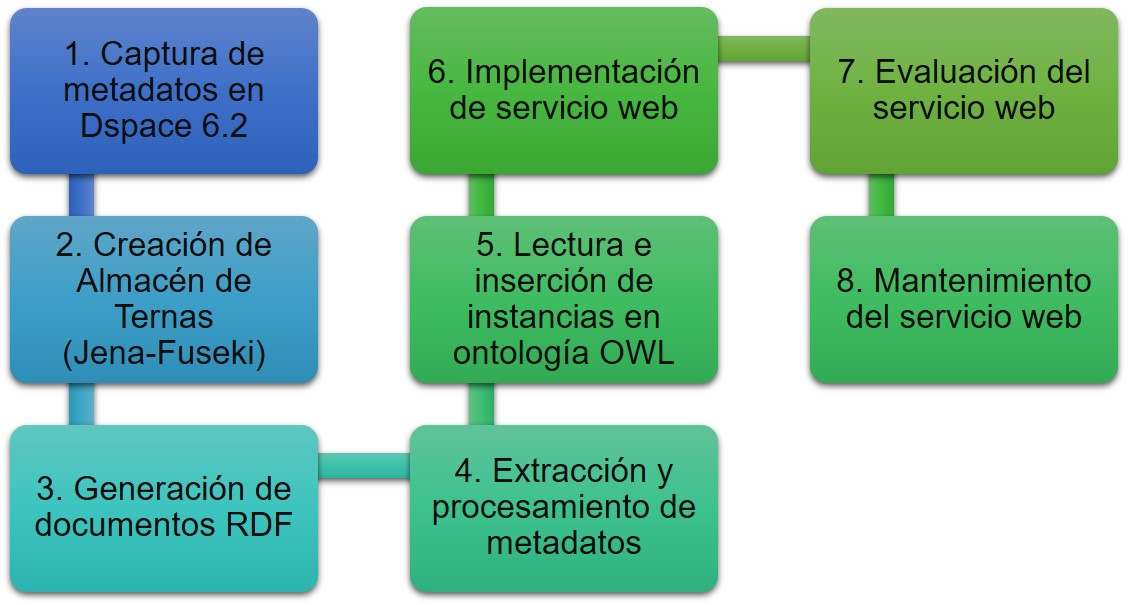
\includegraphics[width=12cm]{figures/etapaResultados.jpg}} 
    \caption{Esquema general de fases para la obtenci\'on de resultados}
    \label{esquemaResultados}
\end{figure}

Adem\'as, se valid\'o el funcionamiento de los servicios tecnol\'ogicos tanto instalados, configurados o desarrollados, a trav\'es de la verificaci\'on de los datos exportados e importados durante los siguientes procesos:

\begin{itemize}
    \item Exportaci\'on de metadatos en formato CSV
    \item Recuperaci\'on de metadatos del almac\'en de ternas en formato RDF
    \item Exportaci\'on de datos a formato JSON
    \item Integraci\'on de instancias a la ontolog\'ia Onto4RI-UPPue en formato OWL
    \item Verificaci\'on del funcionamiento de la interfaz web
\end{itemize}

\subsection{Fase 1. Captura de metadatos en DSpace 6.2}

Dentro de esta etapa se realizaron las siguientes actividades:

\begin{itemize}
    \item Instalaci\'on de una instancia local de la plataforma DSpace versi\'on 6.2, para la realizaci\'on de pruebas emulando las mismas condiciones t\'ecnicas del RI-UPPue
    \item Creaci\'on de una comunidad \textit{Tesis}, Figura \ref{creacionComunidad}
    \item Creaci\'on de la colecci\'on \textit{Maestr\'ia}, Figura \ref{creacionColeccion}
    \item Inserci\'on de once \'items: \textit{metadatos + archivos}, Figura \ref{itemsAgregados}
\end{itemize}{}

\begin{figure}[!ht]
	\centering
	\fbox{
	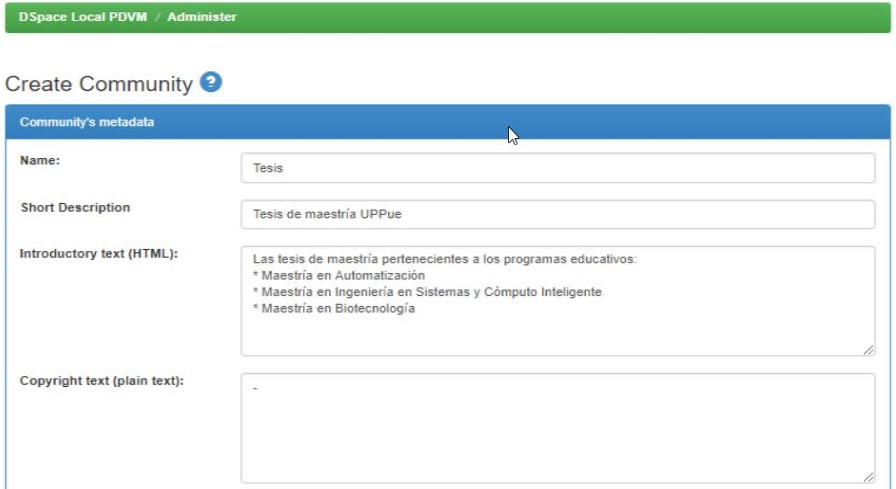
\includegraphics[width=12cm]{figures/creacionComunidad.jpg}} 
    \caption{Creaci\'on de la comunidad de \textit{tesis}}
    \label{creacionComunidad}
\end{figure}

\begin{figure}[!ht]
	\centering
	\fbox{
	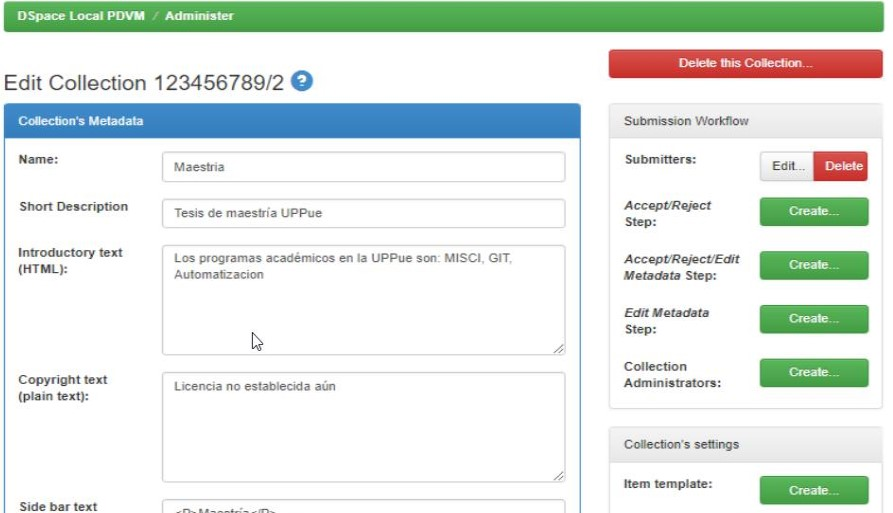
\includegraphics[width=12cm]{figures/creacionColeccion.jpg}} 
    \caption{Creaci\'on de la colecci\'on \textit{maestr\'ia}}
    \label{creacionColeccion}
\end{figure}

\begin{figure}[!ht]
	\centering
	\fbox{
	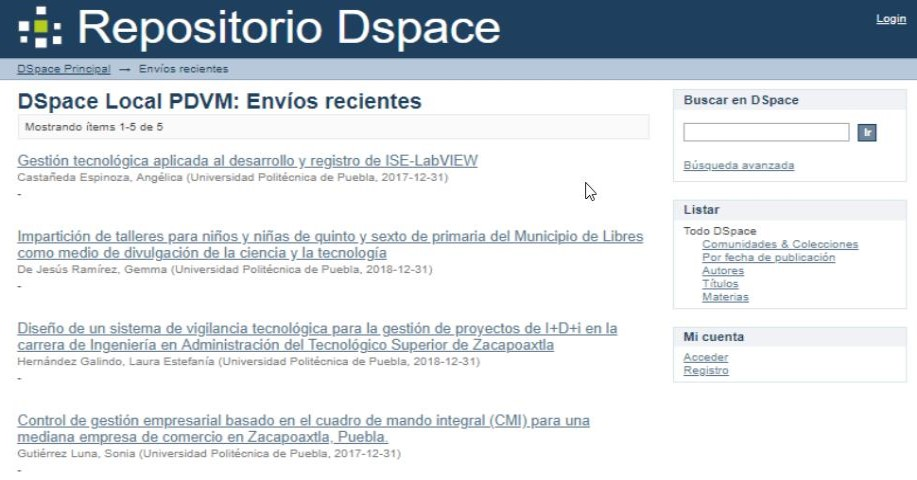
\includegraphics[width=12cm]{figures/itemsAgregados.jpg}} 
    \caption{\'items agregados a la comunidad de \textit{tesis}}
    \label{itemsAgregados}
\end{figure}

\subsection{Fase 2. Creaci\'on de almac\'en de ternas}

Se llev\'o a cabo la instalaci\'on del almac\'en de ternas conforme a las actividades descritas en la Figura \ref{instalacionTriplestore} para la instalaci\'on de los componentes necesarios para habilitar \'este servicio de tipo persistente.

\begin{figure}[!ht]
	\centering
	\fbox{
	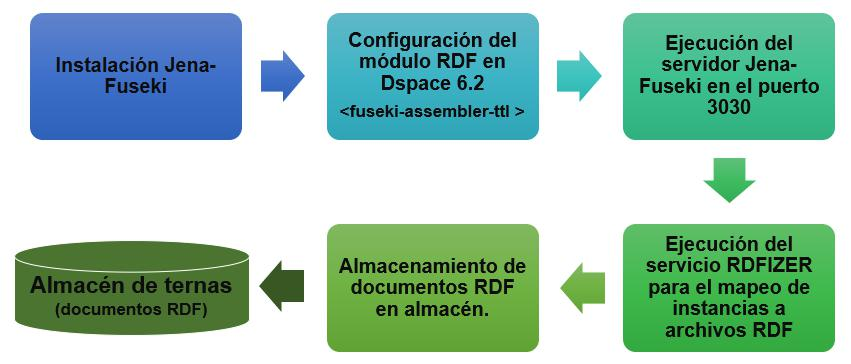
\includegraphics[width=12cm]{figures/InstalacionTripleStore.jpg}} 
    \caption{Implementaci\'on del almac\'en de ternas empleando el servidor Apache Jena Fuseki versi\'on 1.6}
    \label{instalacionTriplestore}
\end{figure}

El \textit{Anexo A} contiene un manual que describe de manera detallada la habilitaci\'on del componente RDF de la plataforma DSpace versi\'on 6.2 a trav\'es de la instalaci\'on del servidor Apache Jena Fuseki versi\'on 1.6, cuya ejecuci\'on se muestra en la Figura \ref{jenaFusekiCorriendo}, lo cual confirma su funcionamiento correcto.

\begin{figure}[!ht]
	\centering
	\fbox{
	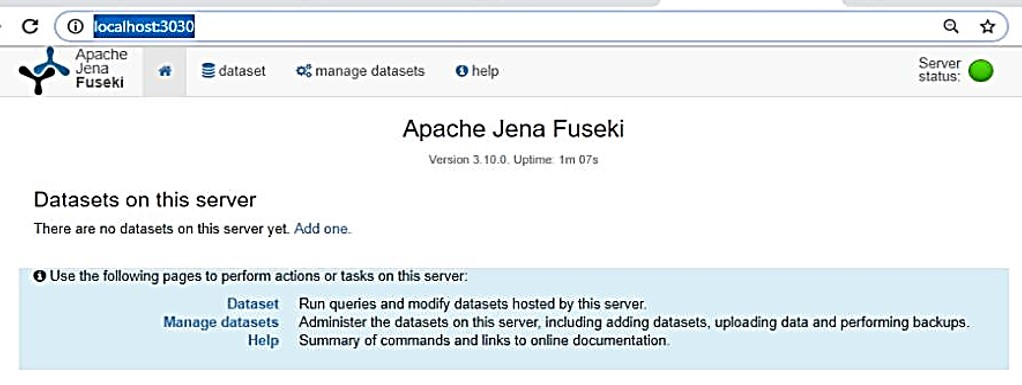
\includegraphics[width=12cm]{figures/ejecuccionJenaFuseki.jpg}} 
    \caption{P\'agina principal del servidor Apache Jena Fuseki corriendo en el servidor local}
    \label{jenaFusekiCorriendo}
\end{figure}

\subsection{Fase 3. Generaci\'on de documentos en RDF}

En esta fase, se realiz\'o la ejecuci\'on del serializador \textit{RDFizer} como se muestra en la Figura \ref{ejecucionRdfizer} para la extracci\'on de metadatos almacenados en DSpace y su migraci\'on al almac\'en de ternas.

\begin{figure}[!ht]
	\centering
	\fbox{
	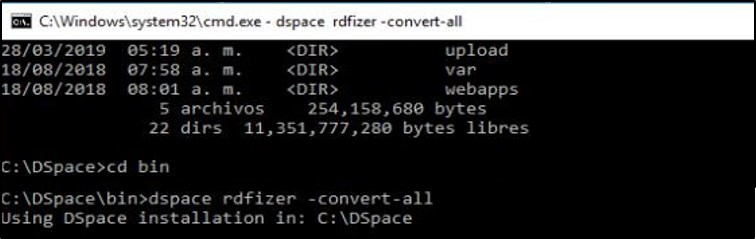
\includegraphics[width=12cm]{figures/ejecucionRDFizer.jpg}} 
    \caption{Ejecuci\'on del serializador \textit{RDFizer}}
    \label{ejecucionRdfizer}
\end{figure}

Para la verificaci\'on de la migraci\'on de \'items almacenados en DSpace al almac\'en de ternas se realiz\'o la verificaci\'on de cada  documento RDF generado, en un conjunto experimental de once instancias agregadas previamente a la plataforma DSpace (ver la Tabla \ref{tablaInstanciasRdf}).

\begin{table}[htbp]
    \begin{center}
    \caption{Actividades de verificaci\'on con instancias migradas a almac\'en de ternas}
    \begin{tabular}{| p{1.5cm}| p{3.5cm} | p{3.5cm} | p{3.5cm} |}
    \hline
    \centering \textbf{No. } & \textbf{Actividad} & \textbf{Resultado esperado} & \textbf{Resultado obtenido} \\
    \hline \hline
    1 & Serializaci\'on de \'items almacenados en DSpace & Once instancias migradas a formato RDF & Once instancias migradas a formato RDF \\ \hline
    2 & Acceso a documento RDF mediante URL & Consulta de once documentos RDF & Consulta de once documentos RDF  \\ \hline
    \end{tabular}
    \label{tablaInstanciasRdf}
    \end{center}
\end{table}

\subsection{Fase 4. Extracci\'on y procesamiento de metadatos}

Se implement\'o un servicio (ver Figura \ref{claseExtraccion}) utilizando la versi\'on 3.6 del lenguaje Python y la librer\'ia RDFlib\footnote{Biblioteca de Python textitleada para trabajar con archivos XLM y RDF} para verificar autom\'aticamente el n\'umero de documentos migrados. La Tabla \ref{casosPruebaMetadatos} muestra los resultados. La figura \ref{metadatosRecuperados} muestra el resultado de ejecutar esta aplicaci\'on.\newline

\begin{table}[htbp]
    \begin{center}
    \caption{Actividades de verificaci\'on con archivos en RDF}
    \begin{tabular}{| p{1.5cm}| p{3.5cm} | p{3.5cm} | p{3.5cm} |}
    \hline
    \centering \textbf{No. } & \textbf{Acci\'on} & \textbf{Resultado esperado} & \textbf{Resultado obtenido} \\
    \hline \hline
    1 & Recuperaci\'on de archivos RDF integrados en el almac\'en de ternas  & Extracci\'on de once tesis & Extracci\'on de once tesis \\ \hline
    2 & Recuperaci\'on de los metadatos de un archivo RDF  & Recuperaci\'on de quince metadatos DCMI & Recuperaci\'on de doce metadatos DCMI, dos metadatos propios de DSpace y tres m\'as \\ \hline
    \end{tabular}
    \label{casosPruebaMetadatos}
    \end{center}
\end{table}

\begin{figure}[!ht]
	\centering
	\fbox{
	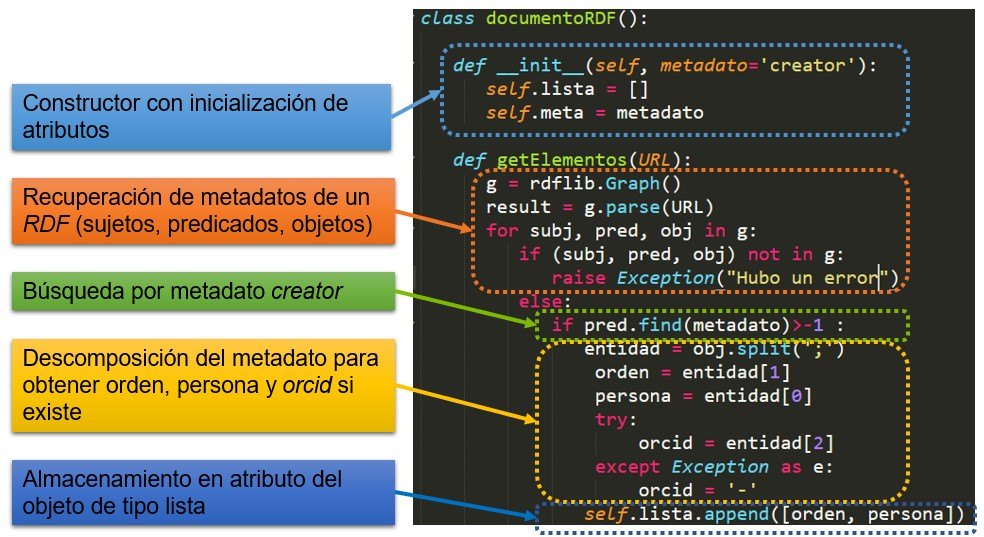
\includegraphics[width=12cm]{figures/claseExtraccion.jpg}} 
    \caption{Descripci\'on de la clase para la extracci\'on de metadatos desde archivo RDF}
    \label{claseExtraccion}
\end{figure}

La Figura \ref{metadatosRecuperados} muestra los metadatos migrados en formato RDF para una tesis.

\begin{figure}[!ht]
	\centering
	\fbox{
	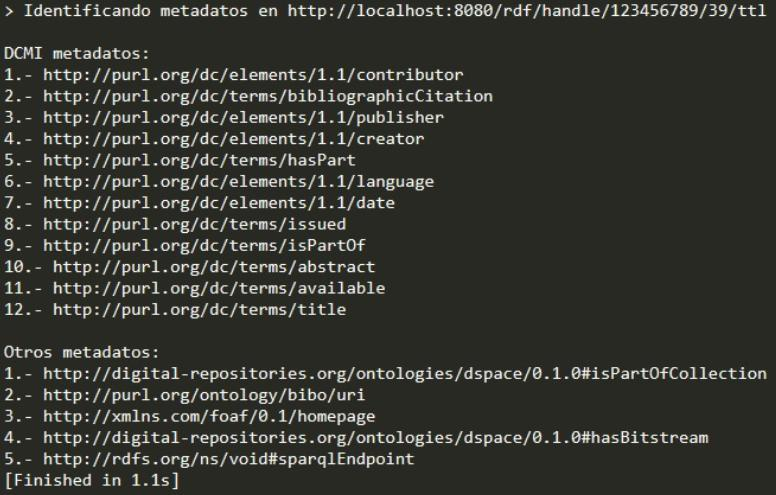
\includegraphics[width=12cm]{figures/metadatosRecuperados.jpg}} 
    \caption{Metadatos recuperados para una instancia del almac\'en de ternas}
    \label{metadatosRecuperados}
\end{figure}

Para verificar los resultados del proceso de migraci\'on, se llev\'o a cabo la revisi\'on de los datos exportados al formato CSV y RDF a un conjunto de prueba experimental (ver la Tabla \ref{casosPruebaInstancias}).\newline

\begin{table}[htbp]
    \begin{center}
    \caption{Actividades de verificaci\'on con archivos CSV}
    \begin{tabular}{| p{1.5cm}| p{3.5cm} | p{3.5cm} | p{3.5cm} |}
    \hline
    \centering \textbf{No. } & \textbf{Actividad} & \textbf{Resultado esperado} & \textbf{Resultado obtenido} \\
    \hline \hline
    1 & Exportaci\'on de instancias en formato CSV & Archivo con once instancias & Archivo con once instancias  \\ \hline
    2 & Exportaci\'on de metadatos en formato CSV  & Archivo con quince metadatos DCMI & Archivo con dieciseis metadatos DCMI y dos metadatos DSpace \\ \hline
    \end{tabular}
    \label{casosPruebaInstancias}
    \end{center}
\end{table}

Los metadatos exportados en CSV son: \textit{id, collection, author, accessioned, available, issued, abstract, provenance, sponsorship, description, citation, uri, iso, publisher, subject, alternative title, title} y \textit{type}.\newline

\subsection{Fase 5. Lectura e inserci\'on de instancias en Onto4RI-UPPue}

El m\'etodo \textit{getroot} permite ubicarse en el nodo ra\'iz de \'arbol, y los m\'etodos \textit{set} y \textit{dump} se emplean para la inserci\'on de nuevos nodos en el cuerpo del documentos, conservando la estructura de las instancias ya existentes en la ontolog\'ia. La Figura \ref{insercionInstancias} muestra un extracto de la implementaci\'on de la inserci\'on de una instancia en la ontolog\'ia.

\begin{figure}[!ht]
	\centering
	\fbox{
	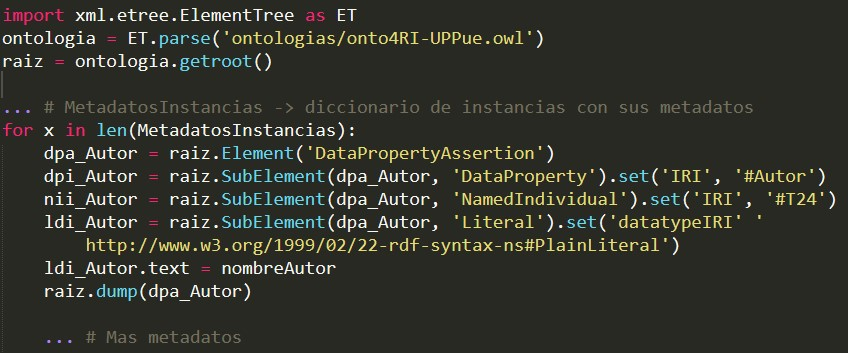
\includegraphics[width=12cm]{figures/insercionInstancia.jpg}} 
    \caption{M\'etodo de inserci\'on de instancias}
    \label{insercionInstancias}
\end{figure}

La Figura \ref{estructuraInstancia} muestra la estructura que deben guardar las instancias agregadas a la ontolog\'ia Onto4RI-UPPue mediante el servicio de integraci\'on.

\begin{figure}[!ht]
	\centering
	\fbox{
	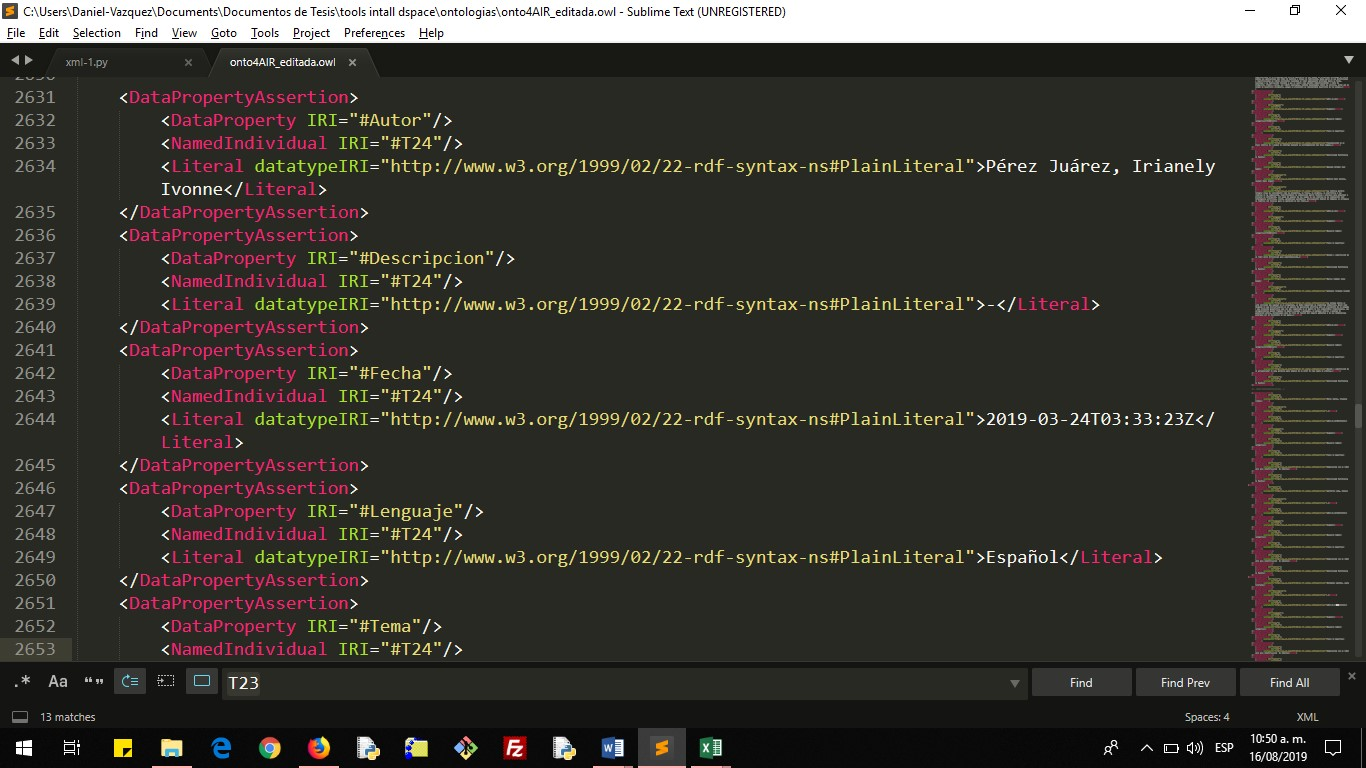
\includegraphics[width=12cm]{figures/instanciaOntologia.jpg}} 
    \caption{Estructura de una instancia agregada por el servicio}
    \label{estructuraInstancia}
\end{figure}

\subsection{Fase 6. Implementaci\'on del servicio web}

La figura \ref{tecnologiasServicio} muestra las tecnolog\'ias empleadas para el desarrollo del servicio web, con lo que el servicio cuenta con las siguientes caracter\'isticas generales:

\begin{itemize}
    \item Responsividad
    \item Validaci\'on HTML
    \item Dinamismo
    \item Accesibilidad
    \item Intuitividad
\end{itemize}{}

El servicio web cuenta con las siguientes secciones:

\begin{itemize}
    \item Inicio
    \item B\'usqueda sem\'antica
    \item Test UX
    \item Exportar
    \item Preguntas frecuentes
    \item Contactos
\end{itemize}{}

Las figuras de la \ref{paginaInicial} a la \ref{paginaContactos} ilustran las secciones contenidas en el servicio web.\newline

La \textbf{p\'agina inicial} muestra un mensaje de bienvenida breve y un listado de los servicios ofrecidos por el servicio.\newline

\begin{figure}[!ht]
	\centering
	\fbox{
	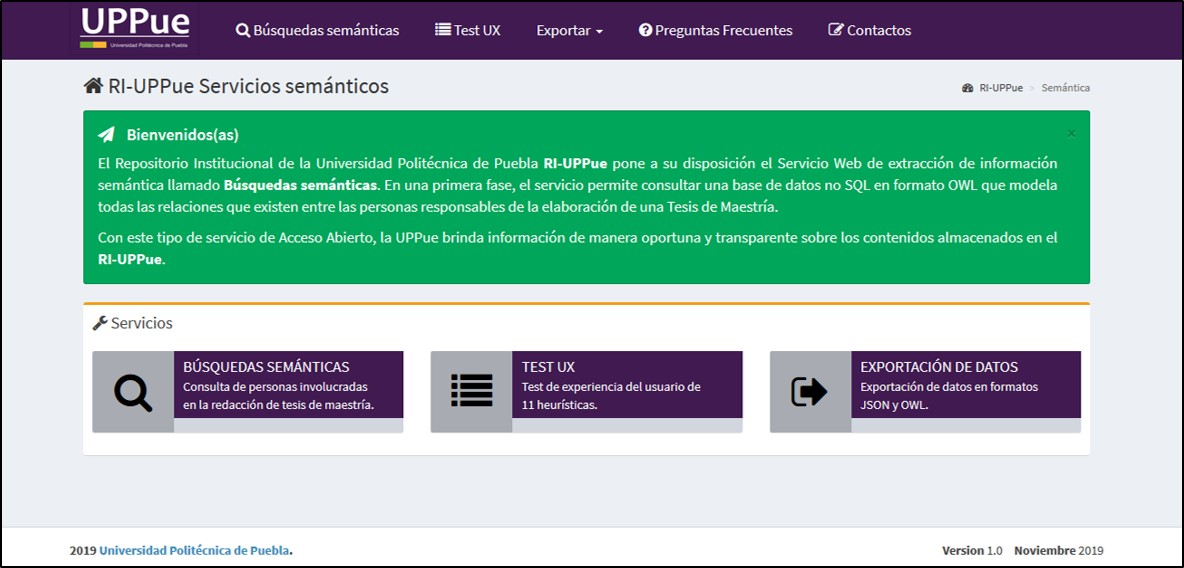
\includegraphics[width=12cm]{figures/paginaInicial.jpg}} 
    \caption{P\'agina inicial del servicio web}
    \label{paginaInicial}
\end{figure}

El servicio de \textbf{b\'usqueda sem\'antica} muestra un panel para realizar b\'usquedas a trav\'es de criterios como \textbf{es autor} y \textbf{es sinodal} que establecen una relaci\'on entre las personas que participaron en la elaboraci\'on de una tesis de maestr\'ia.\newline

\begin{figure}[!ht]
	\centering
	\fbox{
	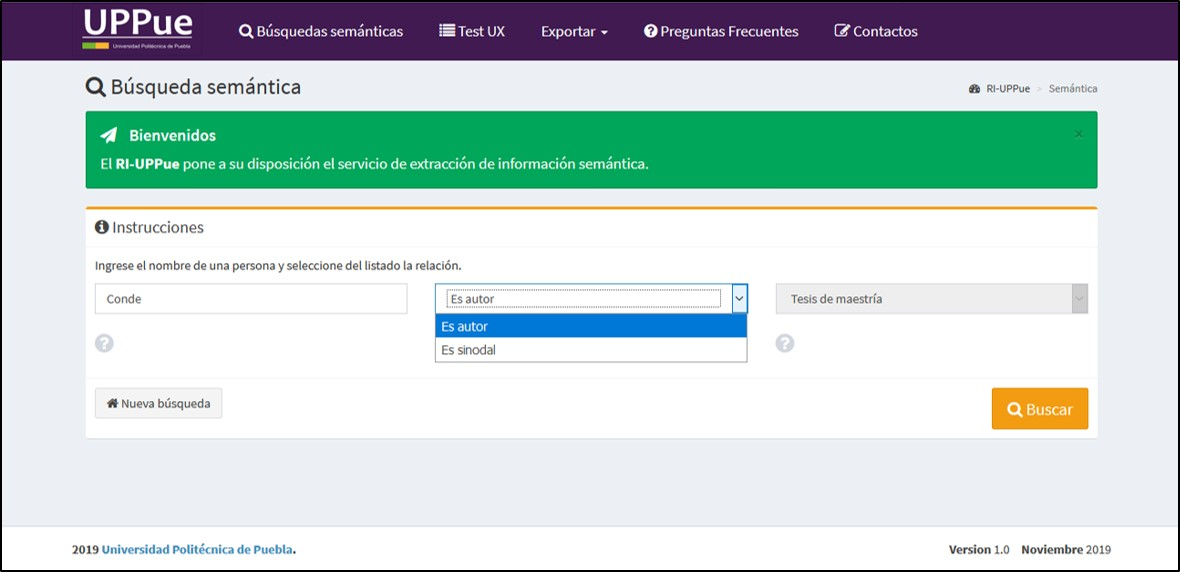
\includegraphics[width=12cm]{figures/paginaBusqueda.jpg}} 
    \caption{Servicio de b\'usqueda sem\'antica}
    \label{paginaSemantica}
\end{figure}

Una vez establecidos los criterios de b\'usqueda y el usuario da click en el bot\'on \textbf{Buscar} en la parte inferior del panel se listan los resultados en forma de tabla.\newline

\begin{figure}[!ht]
	\centering
	\fbox{
	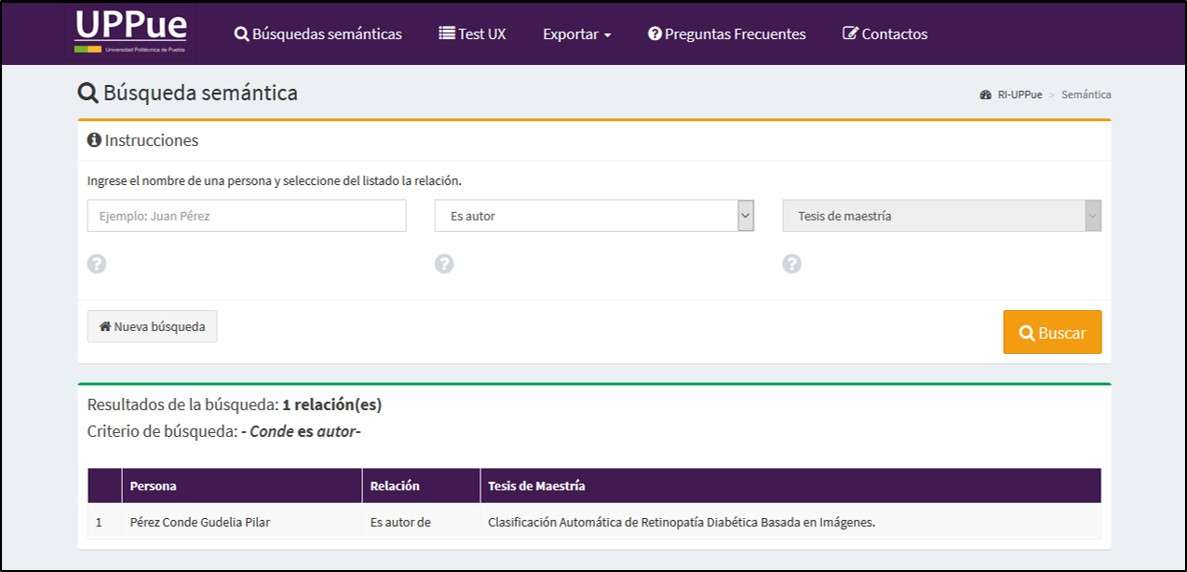
\includegraphics[width=12cm]{figures/paginaResultados.jpg}} 
    \caption{Resultados de la de b\'usqueda sem\'antica}
    \label{paginaResultados}
\end{figure}

El servicio tambi\'en brinda la posibilidad de descargar la ontolog\'ia en dos formatos de intercambio de informaci\'on como lo son \textit{JSON} y \textit{OWL}, que son parseables por cualquier lenguaje de programaci\'on de alto nivel.\newline

\begin{figure}[!ht]
	\centering
	\fbox{
	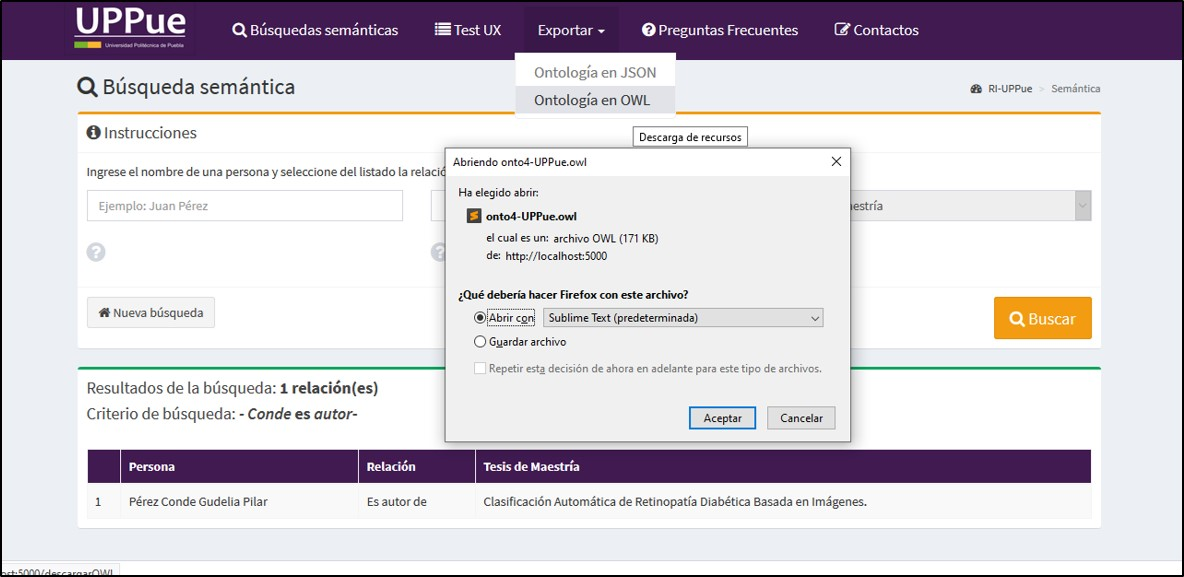
\includegraphics[width=12cm]{figures/paginaExportar.jpg}} 
    \caption{Servicio para la descarga de la ontolog\'ia en formato JSON/OWL}
    \label{paginaExportar}
\end{figure}

De igual manera, se ofrece hay una secci\'on de preguntas frecuentes que el usuario del servicio web puede consultar para conocer m\'as a cerca de los conceptos b\'asicos y terminolog\'ia con la que no se encuentra familizarizado.\newline

\begin{figure}[!ht]
	\centering
	\fbox{
	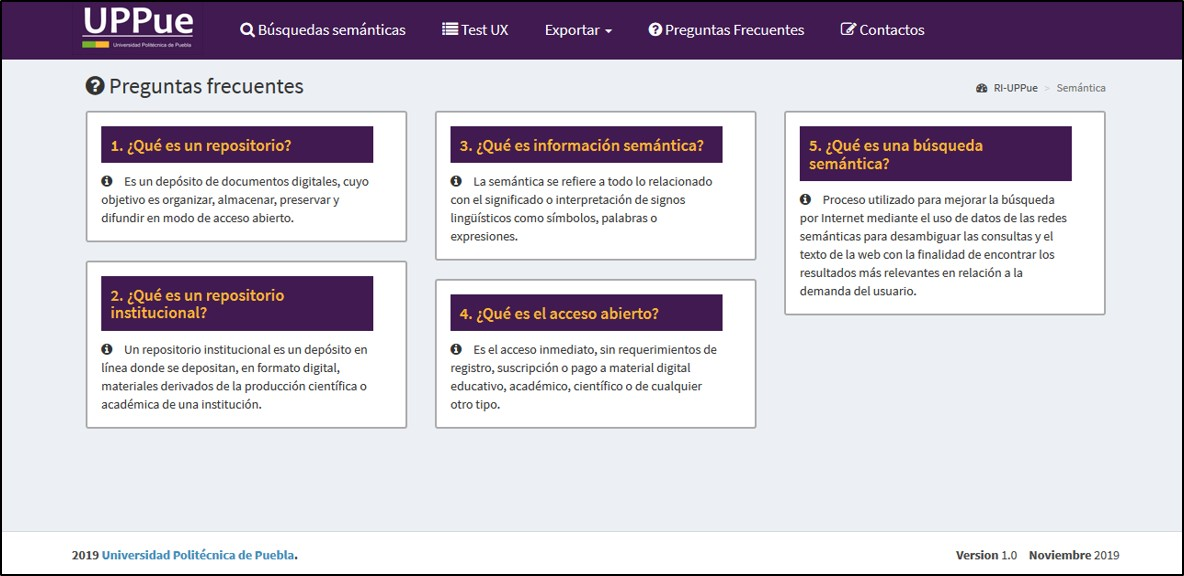
\includegraphics[width=12cm]{figures/paginaPreguntas.jpg}} 
    \caption{P\'agina de preguntas frecuentes}
    \label{paginaPreguntas}
\end{figure}

Finalmente, se anexa una p\'agina con los datos de contactos tanto de la directora de proyecto, como del desarrollador del mismo.\newline

\begin{figure}[!ht]
	\centering
	\fbox{
	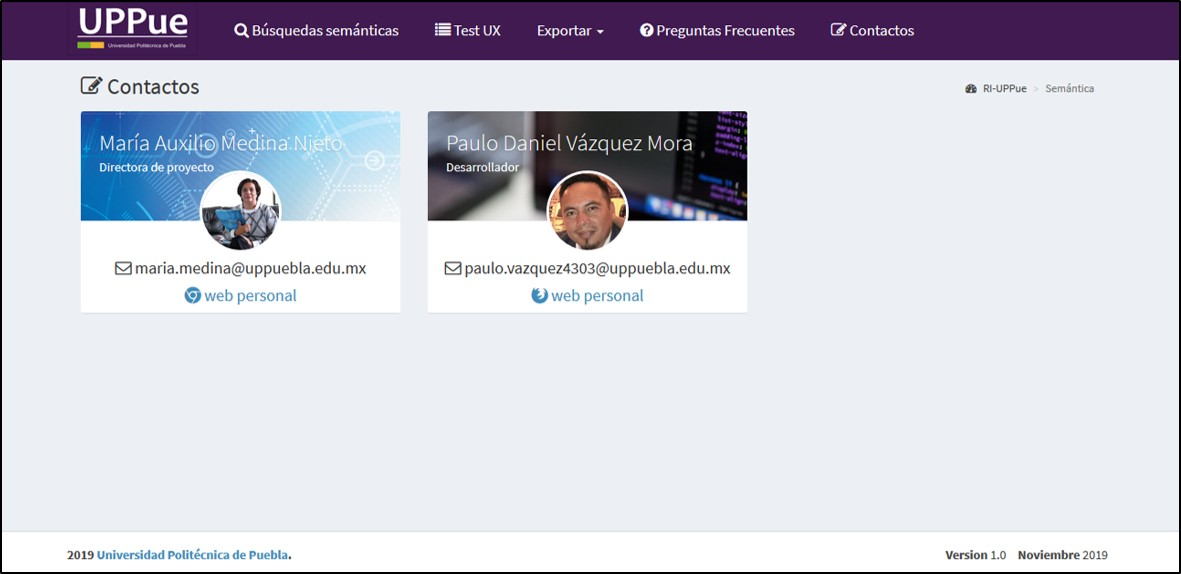
\includegraphics[width=12cm]{figures/paginaContactos.jpg}} 
    \caption{P\'agina de contactos}
    \label{paginaContactos}
\end{figure}

Adem\'as, el servicio web es accesible tanto en equipos de c\'omputo de escritorio y cualquier dispositivo m\'ovil que cuente con conexi\'on a Internet, y para cualquier tipo de sistema operativo, como lo muestra la Figura \ref{vistaMovil}.\newline

\begin{figure}[!ht]
	\centering
	\fbox{
	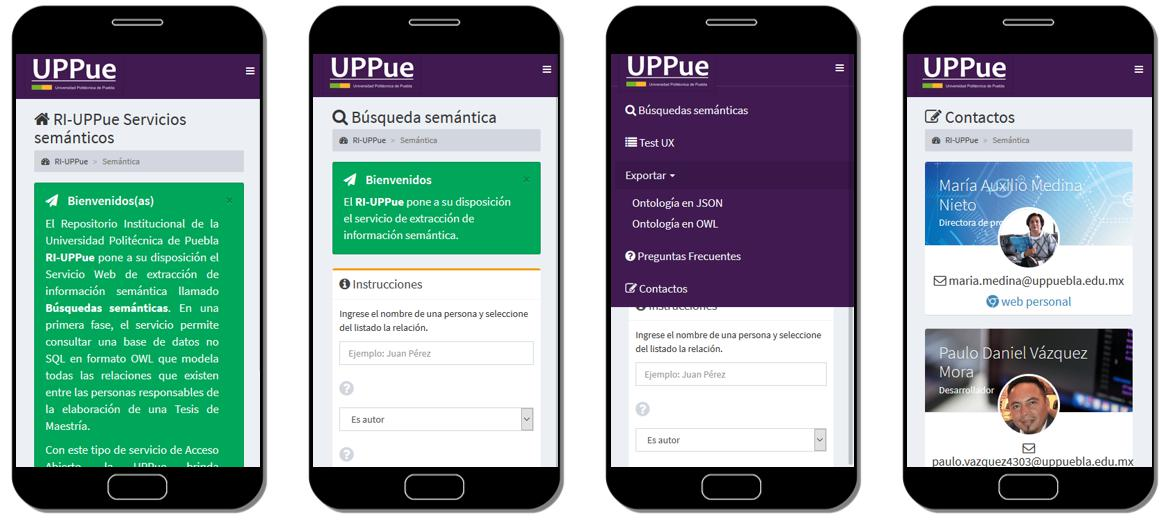
\includegraphics[width=12cm]{figures/vistaResponsiva.jpg}} 
    \caption{Vista responsiva del servicio web a trav\'es de un dispositivo m\'ovil}
    \label{vistamovil}
\end{figure}



\subsection{Fases 7 y 8. Evaluaci\'on y mantenimiento del servicio web}

\subsubsection{Verificaci\'on del proceso de integraci\'on de instancias}

Se realizaron observaciones en el contenido del archivo OWL para identificar las instancias extra\'idas e integradas a la ontolog\'ia mediante el servicio. La Tabla \ref{tablaEvaluacionProtege} muestra los resultados observados.

\begin{table}[htbp]
    \begin{center}
    \caption{Verificaci\'on de instancias agregadas a Onto4RI-UPPue}
    \begin{tabular}{| p{1.5cm}| p{3.5cm} | p{3.5cm} | p{3.5cm} |}
    \hline
    \centering \textbf{No. } & \textbf{Actividad} & \textbf{Resultado esperado} & \textbf{Resultado obtenido} \\
    \hline \hline
    1 & Integraci\'on de nueve instancias de tesis en la ontolog\'ia & Integraci\'on de nueve instancias de tesis en la ontolog\'ia & Integraci\'on de nueve
Instancias de tesis en la ontolog\'ia
  \\ \hline
    2 & Validaci\'on de instancias mediante prot\'eg\'e\footnote{Editor de ontolog\'ias, disponible en \textit{https://protege.stanford.edu/}} & Identificaci\'on de nueve instancias de tesis como “Individuals” dentro de la ontolog\'ia & Identificaci\'on de nueve instancias de tesis como “Individuals” dentro de la ontolog\'ia \\ \hline
    \end{tabular}
    \label{tablaEvaluacionProtege}
    \end{center}
\end{table}

La Figura \ref{instanciaProtege} muestra la integraci\'on de instancias dentro de la ontolog\'ia Onto4RI-UPPue. La secci\'on \textit{Individuals} de prot\'eg\'e muestra las instancias agregadas mediante el servicio bajo la denominaci\'on de T24 hasta T32. Dentro de las propiedades de cada instancia es posible consultar los metadatos que contienen las instancias.

\begin{figure}[!ht]
	\centering
	\fbox{
	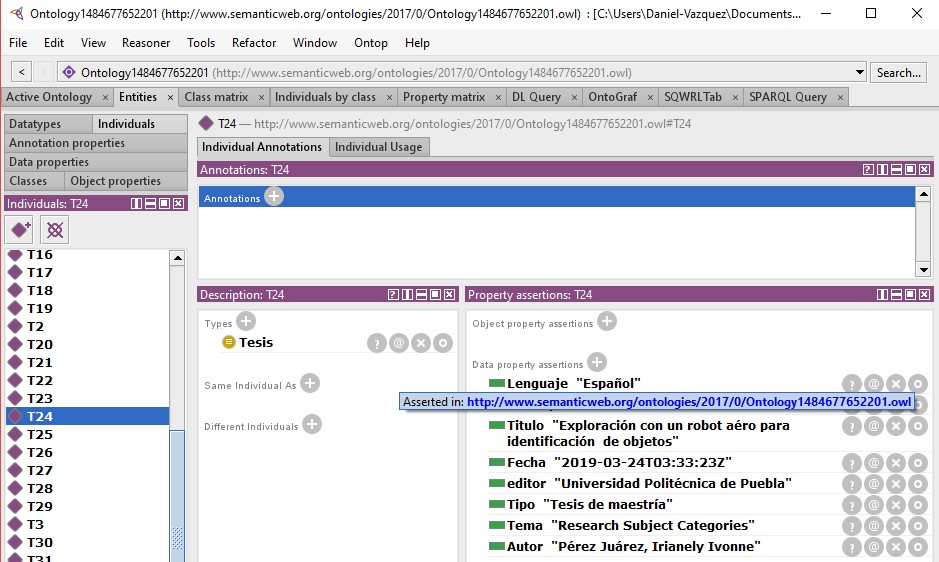
\includegraphics[width=14cm]{figures/instanciasOnto4riUppue.jpg}} 
    \caption{Vista de la instancia T24 agregada por el servicio de integraci\'on}
    \label{instanciaProtege}
\end{figure}

\subsection{Evaluaci\'on de la experiencia del usuario}

Como un servicio complementario, se desarroll\'o una aplicaci\'on web que eval\'ua la experiencia del usuario mediante un cuestionario que considera las once heur\'isticas propuestas por \cite{OnceHeuristicas}. La figura \ref{testUX} muestra la pantalla principal del test.\newline

\begin{figure}[!ht]
	\centering
	\fbox{
	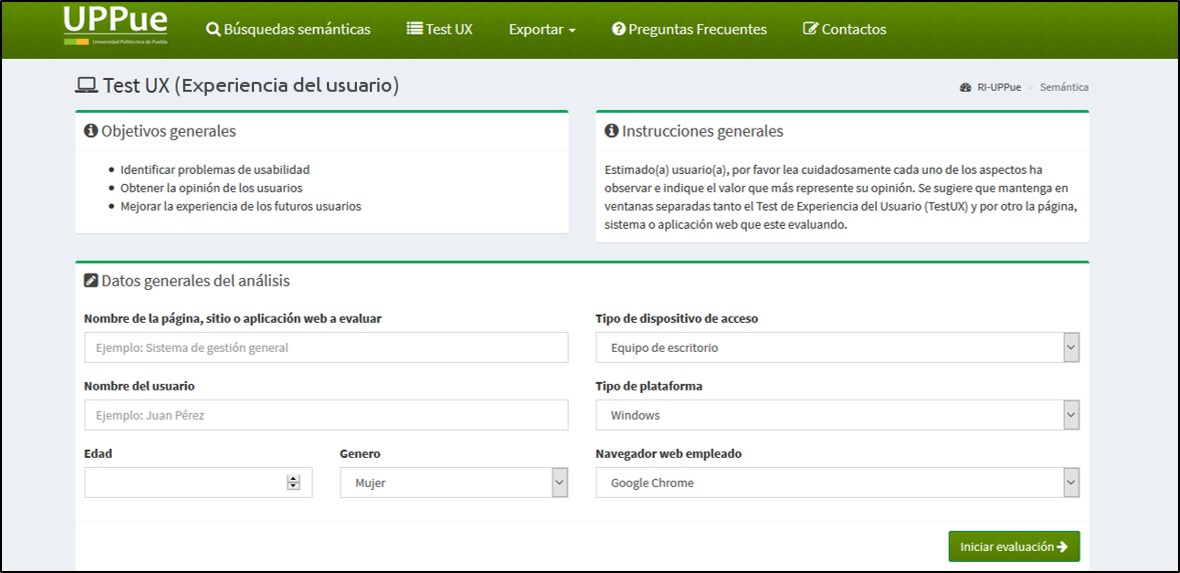
\includegraphics[width=14cm]{figures/testUX_corregida.jpg}} 
    \caption{Pantalla principal del TestUX}
    \label{testUX}
\end{figure}

Para la evaluaci\'on del servicio web participaron diecis\'eis usuarios con las siguientes caracter\'isticas generales:

\begin{itemize}
    \item 6 mujeres y 10 hombres
    \item Las edades de los usuarios est\'an en el rango de los 21 y 24 a/~{n}os
    \item Todos alumnos de la carrera de ingenier\'ia en inform\'atica, pr\'oximos a egresar.
    \ 
\end{itemize}{}

Cabe resaltar que seg\'un \cite{CincoEstrellas} y \cite{OnceHeuristicas}, s\'olo se requiere de cinco personas para poder realizar la evaluaci\'on de la experiencia del usuario, con lo que se excede del n\'umero sugerido por los autores antes mencionados.\newline

La evaluaci\'on consisti\'o en una serie de afirmaciones, en las cuales los usuarios indicaron a trav\'es de una escala Likert de cinco grados, el nivel de satisfacci\'on con las caracter\'isticas , elementos o funcionalidades que el servicio web deber\'ia contar. Las escalar consideradas son las siguientes:

\begin{itemize}
    \item No aplica (0)
    \item Totalmente insatisfecho (1)
    \item Muy insatisfecho (2)
    \item Satisfecho (3)
    \item Muy satisfecho (4)
    \item Totalmente satisfecho (5)
\end{itemize}{}

Las figuras \ref{evaluacionResultados} y \ref{evaluacionResultadoGral}  muestran los resultados obtenidos en la evaluaci\'on por cada una de las heur\'isticas y de manera general respectivamente.\newline

\begin{figure}[!ht]
	\centering
	\fbox{
	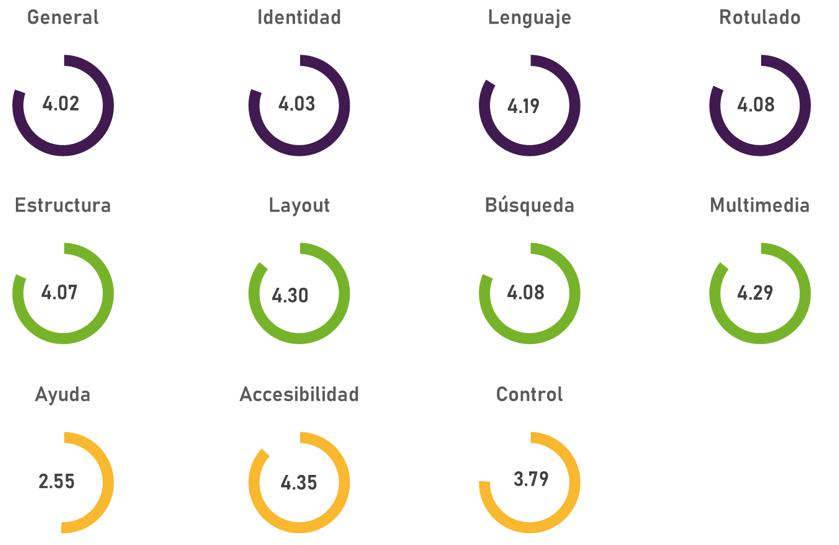
\includegraphics[width=14cm]{figures/evaluacionResultadosHeuristicas.jpg}} 
    \caption{Resultados de la evaluaci\'on del servicio web}
    \label{evaluacionResultados}
\end{figure}

\begin{figure}[!ht]
	\centering
	\fbox{
	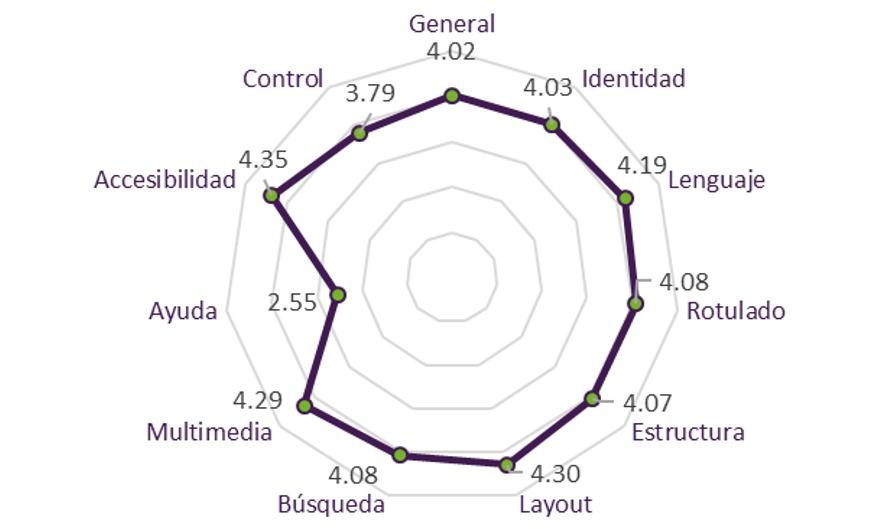
\includegraphics[width=14cm]{figures/evaluacionResultadoGral.jpg}} 
    \caption{Resultado general de la evaluaci\'on del servicio web}
    \label{evaluacionResultadoGral}
\end{figure}

Derivado de los resultados mostrados en figuras \ref{evaluacionResultados} y \ref{evaluacionResultadoGral} se concluy\'o que la heur\'istica mejor evaluada fue la de accesibilidad y la peor fue ayuda.\newline

El promedio de las calificaciones obtenidas fue de \textbf{4} por lo que se concluye que el usuario se siente \textbf{muy satisfecho} con el servicio web.\newline

La figura \ref{evaluacionUsuarios} muestra evidencia fotogr\'afica de los usuarios que realizaron la evaluaci\'on del servicio web.\newline

\begin{figure}[!ht]
	\centering
	\fbox{
	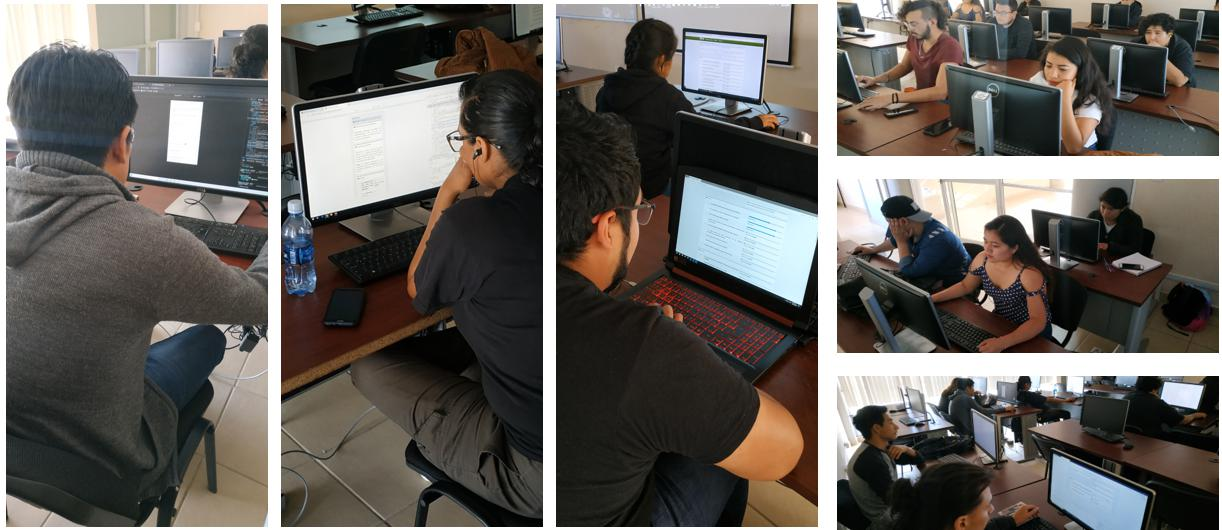
\includegraphics[width=14cm]{figures/evaluacionAlumnos.jpg}} 
    \caption{Usuarios realizando la evaluaci\'on del servicio web}
    \label{evaluacionUsuarios}
\end{figure}

\subsection{Mantenimiento del servicio web}

A trav\'es de la aplicaci\'on de la evaluaci\'on de experiencia del usuario se identificaron las siguientes \'areas de oportunidad: 

\begin{itemize}
    \item El usuario requiere mayor n\'umero de elementos de ayuda.
    \item El usuario requiere una mejor retroalimentaci\'on sobre las cosas que est\'an sucediendo con los servicios ofrecidos.
\end{itemize}{}

Por lo anterior, se implementaron diferentes elementos de ayuda contextual y mensajes de retroalimentaci\'on que permitieran al usuario a identificar correctante el tipo de acciones que deber\'ia llevar a cabo en cada secci\'on. las figuras \ref{ayudaContextual}, \ref{ayudaMensaje} y \ref{ayudaNavegacion} muestran los elementos implementados para atender las necesidades identificadas en la evaluaci\'on.\newline

\begin{figure}[!ht]
	\centering
	\fbox{
	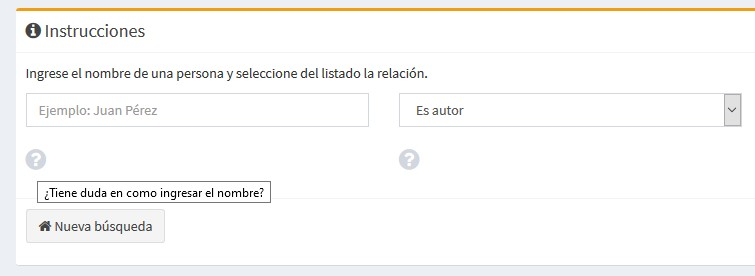
\includegraphics[width=14cm]{figures/mantto1.jpg}} 
    \caption{Iconos para ayuda contextual}
    \label{ayudaContextual}
\end{figure}

\begin{figure}[!ht]
	\centering
	\fbox{
	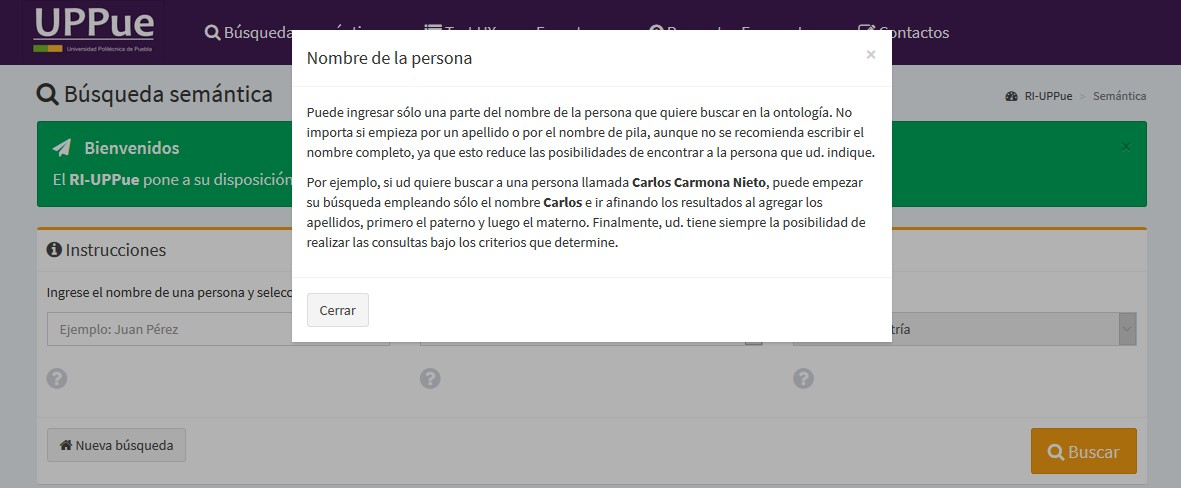
\includegraphics[width=14cm]{figures/mantto2.jpg}} 
    \caption{Mensaje para la descripci\'on detallada de elementos y ejemplos de uso}
    \label{ayudaMensaje}
\end{figure}

\begin{figure}[!ht]
	\centering
	\fbox{
	
\includegraphics[width=14cm]{figures/mantto3.jpg}} 
    \caption{Mensajes contextuales sobre los servicios ofrecidos en la barra de navegaci\'on}
    \label{ayudaNavegacion}
\end{figure}

